%Use pdfLaTeX to compile

\documentclass[12pt,a4paper]{report}
\usepackage[pdftex]{graphicx}
\usepackage{titletoc} 
\usepackage{fancyhdr}   
\usepackage[a4paper,pdftex]{geometry}	
\usepackage[english]{babel}
\usepackage{xcolor} 
\usepackage{enumerate}
\usepackage{fix-cm} 
\usepackage[notlof]{tocbibind}
\usepackage{amsmath}
\usepackage{listings}

\bibliographystyle{ieeetr}  
\usepackage[toc,page]{appendix}

\begin{document}
\begin{titlepage}
\begin{center}

\includegraphics[scale=1.5]{CoverSheet}\\
\bf{ DEPARTMENT OF ELECTRICAL AND ELECTRONIC ENGINEERING }
\end{center}

\vspace{18mm}
 \begin{center}
 \begin{Large}
 {EEE311 Final Year Project}\\ 
 \vspace{2.0cm}
 \bf{Title of your FYP Project}
 \end{Large}
 \end{center} 
\vspace{2.0cm}

  \begin{center}
  \begin{large}
  In Partial Fulfillment\\
  of the Requirements for the Degree\\
  Bachelor of Engineering\\
   \vspace{3.0cm}
     \begin{tabular}{r@{ }l} 
       Student Name : & Your Name\\ 
       Student ID : & Your student ID\\ 
       Supervisor : &  Your supervisor's name\\ 
       Assessor : & Your accessor's name \\
    \end{tabular}
  \end{large}
  \end{center}
\clearpage
\end{titlepage}

\abstract{Write your abstract here}

\tableofcontents


\quad 
\setcounter{page}{1}
\chapter{Introduction}
This is the introduction.  Do ensure that you include relevant references in under this section.  Some examples of references are found in \cite{ting2013resource,jayaprakasam2013pareto}. This is explained in \cite{ting2013resource, jayaprakasam2013genetic,jayaprakasam2013pareto}.  This is just an example, the variable $x$. This is described in
\begin{equation}
	E=mc^2 \nonumber
\end{equation}

\[
E=mc^2
\]

\begin{eqnarray}
	P_1 &=& 5 \\
	P_2 &=& 6 \{ 7 \nonumber\\
	P_3 &=& 57               \& \quad 46\\
	P_4 &=& \frac{1}{2}
\end{eqnarray}

This is $5\:$V.  This is $\mathbf{N}$


\chapter{Methodology} 
Describe your method here: the Asymptote and Matlab programming languages that you use in this project.

\section{Asymptote}
This is for Asymptote

\section{Matlab}
This is for Matlab kdflk Figure \ref{fig1}.



\begin{figure}[ht!] 
\begin{center}
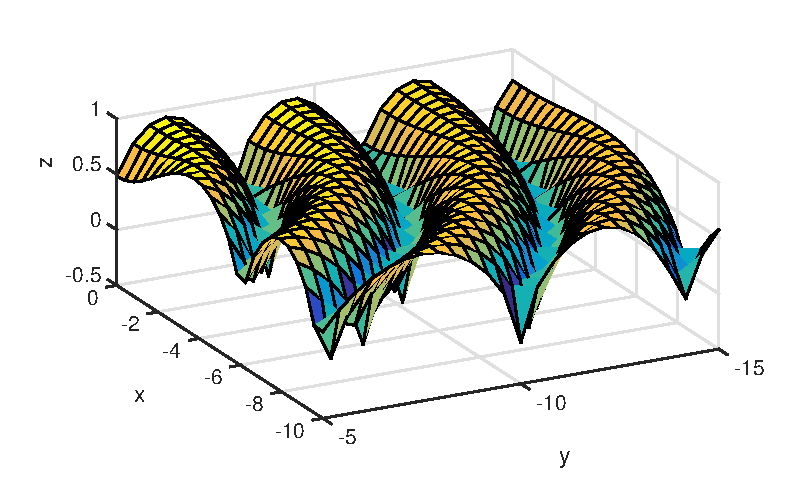
\includegraphics[scale=1.2]{f1}
\caption{The tracing chip}
\label{fig1}
\end{center}
\end{figure}


\section{Item List}
Here are three examples of item lists:
\begin{itemize}\itemsep -2pt
\item This is item 1
\item This is item 2
\item This is item 3
\item This is item 4
\end{itemize}

\begin{enumerate}\itemsep -2pt
\item This is one
\item This is two
\item This is three
\end{enumerate}

\begin{enumerate}[1.]\itemsep -2pt
\item This is one
\item This is two
\item This is three
\end{enumerate}

\begin{itemize}
	\item sjdkf sdf
	\item lksdjfklsj sd
	\item f ksdjfk sdfkjk sdf
	\item skldfjk sdfsdfs
\end{itemize}

\begin{description}
	\item [One] ksjdk sdkfk
	\item [second] skdfk sdkfj kjsdfk ksjdfkjkksdfkj 
	\item [third] k ksdfjksdj fkjskdfjksdf
\end{description}

\chapter{Result and Discussion}
Make sure you write something here before you begin with the subsection. 

\section{Figure}
A sample of figure is given as Figure \ref{fig1}

\section{Table}
Include table whenever necessary.  An example is given as Table 

\section{Justification via Matlab}
This is where you can prove that the results obtained are accurate and valid

\section{Comparison}
Comparison is also necessary to justify your results.


\chapter{Improvement}
Describe the improvements that you have done in this project.

\chapter{Conclusion}
Here comes the conclusion!

%\begin{thebibliography}{x}
%%\bibitem{avinash11pc} Avinash (2011, Dec.25). PC Controlled Robot [Online]. Available: http://extremeelectronics.co.in/avr-projects/pc-controlled-robot/
%
%\bibitem{wendlandt05indoor} Wendlandt, K.; Berhig, M.; Robertson, P., "Indoor localization with probability density functions based on Bluetooth," Personal, Indoor and Mobile Radio Communications, 2005. PIMRC 2005. IEEE 16th International Symposium on, vol.3, no., pp.2040,2044 Vol. 3, 11-14 Sept. 2005
%
%\end{thebibliography}


\bibliographystyle{IEEEtran}
\bibliography{ref}

\begin{appendices}
\begin{verbatim}
The whole codes:

#include<IRremote.h>
#include<Wire.h>
#include <LiquidCrystal_I2C.h>
LiquidCrystal_I2C lcd(0x27, 16, 2);



int RECV_PIN = 11; 
IRrecv irrecv(RECV_PIN); 
decode_results results; 

int AIN1 = 6; //PWMA
int AIN2 = 5; //DIRA
int BIN1 = 10; //PWMB
int BIN2 = 9; //DIRB
int sensorPin = A0; 
int ledPin = 13; 
int sensorValue = 0; 



int melody[] = {330, 330, 330, 262, 392, 200, 280};
int noteDurations[] = {8, 4, 4, 8, 4, 4, 6};

void setup() 
{
pinMode(AIN1, OUTPUT);
pinMode(AIN2, OUTPUT);
pinMode(BIN1, OUTPUT);
pinMode(BIN2, OUTPUT);
pinMode(ledPin, OUTPUT);
Serial.begin(9600);


}
}
\end{verbatim}

%Example of Matlab code, remember to include "listings" package
\begin{lstlisting}[language={MATLAB}, keywordstyle=\color{blue!70},commentstyle=\color{green!40!black},frame=shadowbox, rulesepcolor=\color{red!20!green!20!blue!20},basicstyle=\footnotesize]
%Justification via Matlab of function 36%
clc;clear;
syms x y Fx Fy A B C D;
z=100*(x-y^2)^2+(1-x)^2+10.1*(y-1)^2
Fx=diff(z,x)
Fy=diff(z,y)
S=solve(Fx,Fy);
x1=S.x
y1=S.y
A=diff(z,x,2)
B=diff(diff(z,x),y)
C=diff(z,y,2)
D=A*C-B^2
D1=subs(subs(D,'x',x1(1)),'y',y1(1))
A1=subs(subs(A,'x',x1(1)),'y',y1(1))
Z1=subs(subs(z,'x',x1(1)),'y',y1(1))
\end{lstlisting}

\end{appendices}
\end{document}
